\chapter{Wstęp}

%TODO Tutaj poszę jednak kilka ogólnych zdań o ADAS (co to jest), pojazdach autonomicznych i roli algorytmów wizyjnych.


\section{Cele i założenia}

Celem niniejszej pracy było stworzenie aplikacji umożliwiającej testowanie algorytmów wizyjnych za pomocą symulatora ciężarówki.
Rozwiązanie to mogłaby być wykorzystane w ramach ćwiczeń laboratoryjnych poruszających problematyką systemów wizyjnych stosowanych w pojazdach autonomicznych prowadzonych w ramach kierunku Automatyka i Robotyka na Akademii Górniczo-Hutniczej.

\section{Istniejące systemy}
%TODO To też jest zbyt "skrome"
Aplikacje służące do testowania algorytmów wizyjnych są używane w przemyśle. 
Obecnie produkowane samochody są wyposażone w systemy, które bazując na widoku z kamery pomagają prowadzić samochód. 
Testowanie tych algorytmów jest niezwykle istotne, ponieważ niewykrycie błędów może prowadzić do katastrofalnych skutków, w tym potencjalnej śmierci człowieka. 
Przykładowo niewystarczające testowanie algorytmów w komercyjnym samochodzie Tesla 3 doprowadziło do śmiertelnego wypadku, ponieważ tzw. ,,autopilot'' nie wykryły poprawnie naczepy ciężarówki.
%TODO Tu nieco zmieniłem, bo wbrew temu co się mówi Tesla w dokumentach nie twierdzi, że to rozwiazanie autonomiczne, tylko autopilot (zabawka, którą trzba nadzorować)

\section{Zawartość pracy}

Rozdział drugi rozpoczyna się opisem poziomów autonomiczności samochodów. 
Zawarte w nim jest porównanie w odniesieniu do stosowanych systemów wizyjnych i innych asystentów jazdy. %TODO styl. "porównanie" w odniesieniu..
Następnie opisane są wybrane algorytmy cyfrowego przetwarzania obrazów takie jak: detekcja pasa ruchu, detekcja świateł drogowych, wykrywanie znaków oraz detekcja samochodu poprzedzającego. %TODO to raczej są systemy wizyjne dla PA/ADAS.
Opis jest oparty na uznanych w świecie naukowym artykułach. %TODO może Opracowano go na podstawie przeglądu publikacji naukowych.
Rozdział kończy krótki opis podstawowych operacji cyfrowego przetwarzania obrazów, których wyjaśnienie uznano za istotne z uwagi na ich częste stosowanie w systemach wizyjnych pojazdów autonomicznych.

Następny rozdział zawiera opis zrealizowanego systemu. 
Na początku dokonana jest ewaluacja dostępnych symulatorów jazdy wraz z uzasadnieniem wyboru Euro Truck Simulator 2. 
Kolejno opisana została architektura zaimplementowanej aplikacji. 
W~następnej części omówiono przykładowe algorytmy zaimplementowane w celu przetestowania i weryfikacji aplikacji stworzonej w ramach pracy. 
Końcowa część to sprawdzenie wydajności aplikacji w różnych sytuacjach.

Ostatni rozdział zawiera krótkie podsumowanie oraz ocenę przydatności aplikacji do prowadzenia zajęć dydaktycznych.

%TODO Koniec sprawdzania TK

\chapter{Systemy wizyjne w pojazdach autonomicznych}
Współczesne pojazdy autonomiczne wykorzystują w szerokim zakresie systemy wizyjne do analizy otoczenia. Jednym z pierwszych zastosowań algorytmów cyfrowego przetwarzania obrazów była detekcja pasa ruchu, która nie służyła do sterowania samochodem, lecz miała za zadanie wspomagać kierowcę w sytuacjach zmęczenia lub utraty koncentracji. Wraz z rozwojem technologii pojazdów autonomicznych, zaawansowanie systemów wizyjnych rosło od wspomnianej kontroli pasa ruchu, poprzez rozpoznawanie znaków drogowych i świateł ulicznych, na detekcji pieszych kończąc. Ważnym elementem o którym należy wspomnieć, że istotne znaczenie, oprócz algorytmów detekcji, ma sposób interpretacji danych odczytanych z otoczenia. W kolejnych podrozdziałach zostaną opisane algorytmy wizyjne, które mogłyby być zastosowane w systemach w pojazdach autonomicznych. 

\section{Poziomy autonomiczności}

Całość systemów, które wspomagają kierowcę w trakcie jazdy nazwano ADAS (Advanced Driver Assistance Systems). Aby usystematyzować  i podzielić poziom wpływu systemów na jazdę wprowadzono poziomy autonomiczności jazdy.

\begin{figure}
  \centering
  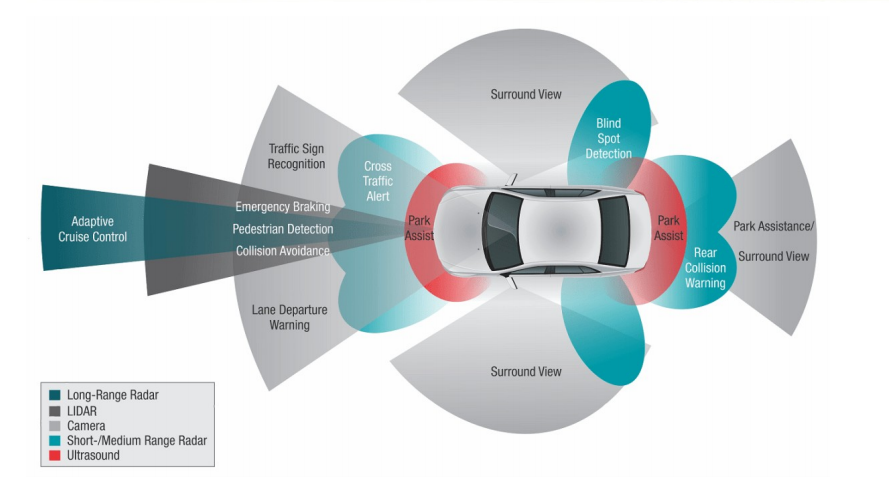
\includegraphics[width=13cm]{img/systemy_autonomiczne_ogolnie.png}
  \caption{Ogólny schemat kamer i radarów we współczesnych pojazdach autonomicznych\cite{S1}}
  \label{fig:kamery_i_radary}
  % https://aindustryreports.com/2019/05/23/advanced-driver-assistance-system-sensor-market-technological-innovations-in-north-america-to-boost-regional-market-attractiveness-through-2026/
\end{figure}

Na rysunku \ref{fig:kamery_i_radary} daje się zauważyć znaczna liczba kamer i radarów wspomagająca kierowcę. Powszechną techniką jest stosowanie redundancji w krytycznych systemach, co jest regulowane poprzez normy ADAS (Advanced Driver Assistance Systems)

\subsection{Poziom zerowy - brak autonomiczności}
Obecnie większość samochodów na drodze zawiera się w tym poziomie. Człowiek wpływa na jazdę, chociaż mogą pojawiać się proste systemy, które mogą pomóc kierowcy np. system awaryjnego hamowania. Dopóki nie wpływa on na tor jazdy, nie jest to system autonomiczny. Innym przykładem jest system ABS, który również nie jest systemem, który zapewniałby autoomiczność pojazdowi. Służy on poprawie bezpieczeństwa i jego działanie opiera się tylko na odczycie danych z czjujników niezależnie od aktualnej sytuacji na drodze i wokół pojazdu.

\subsection{Poziom pierwszy - asysty kierowcy}
Jest to najniższy poziom autonomiczności. Auto posiada pojedynczy system wspomagania kierowcy taki jak sterowanie lub przyspieszanie (tempomat). Adaptacyjny tempomat, czyli system, który zachowuje bezpieczny dystans od poprzedzającego pojazdu kwalifikuje się jako poziom pierwszy, ponieważ człowiek kontroluje pozostałe aspekty jazdy samochodem takie jak kierowanie i hamowanie.

\subsection{Poziom drugi - częściowa automatyzacja jazdy samochodem}
Oznacza zaawansowane asysty kierowcy. Samochód może sam kontrolować zarówne sterowanie i przyspieszanie oraz hamowanie. Jest w stanie jechać samodzielnie, lecz wymaga ciągłej obecności kierowcy za kierownicą, który może w każdej chwili przejąć kontrolę nad samochodem. Obecnie stosowane systemy jazdy autonomicznej takie jak np. Tesla Autopilot kwalifikują się jako poziom drugi.

\begin{figure}
  \centering
  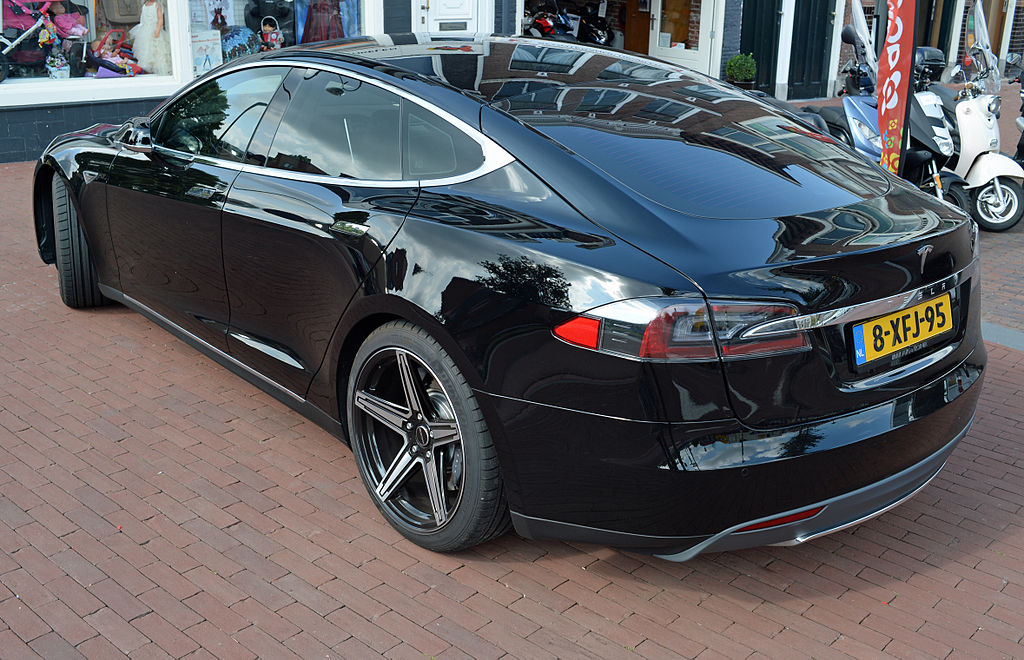
\includegraphics[width=12cm]{img/tesla.jpg}
  \caption{Tesla Model S - pierwszy samochód z drugim poziomem zaawansowania systemów wspomagania kierowcy (\textit{źródło: Wikipedia})}
  \label{fig:teslas}
  % https://pl.wikipedia.org/wiki/Tesla_Model_S#/media/Plik:2014_Tesla_Motors_Model_S_(rear_view)_Netherlands.jpg
\end{figure}

\subsection{Poziom trzeci}
Różnica w stosunku do poziomu drugiego jest subtelna. Samochód posiada możliwość detekcji otaczającego go środowiska i na podstawie zgromadzonych informacji samodzielnie podejmować decyzje. System jest jednak wciąż zależny od człowieka, który musi pozostać czujny i być w stanie zareagować, gdy system nie będzie w stanie podjąć decyzji. W 2019r. Audi wprowadziło model A8, który zapowowiadano jako pierwszy samochód poziomu trzeciego. System Traffic Jam Pilot bazując na danych z lidaru oraz kamer zapewniał autonomiczną jazdę w korkach. Problemem okazało się nieprzygotowanie prawne. W Stanach Zjednoczonych stosowanie tego systemu było zabronione, więc samochód w okrojonej wersji sprzedawano jako pojazd autonomiczny drugiego poziomu. W Europie samochód pojawił się z zaimplementowaną funkcjonalnością asystenta jazdy w korku.

\subsection{Poziom czwarty}
Poziom czwarty zapewnia to czego brakowało w niższych poziomach, a więc może interweniować jeśli coś pójdzie nie tak (np. nagły wypadek, pęknięcie opony). Te samochody nie wymagają akcji w człowieka w znakomitej większości sytuacji, jednak człowiek zawsze jest w stanie przejąć kontrolę. Podobnie jak w poziomie trzecim problemem okazały się ograniczenia prawne. Samochody te mogą z reguły poruszać się na ograniczonym obszarze. Obecnie w fazie testów są samochody takie jak Waymo lub NAVYA

\subsection{Poziom piąty - pełna autonomia}
Samochody nie wymagają uwagi człowieka. Najprawdopobniej nie będą wyposażone w kierownicę ani pedały. Będą w stanie jechać gdziekolwiek i robić to co jest w stanie zrobić doświadczony kierowca. Samochody te są obecnie w stanie wczesnych testów, jednak można się spodziewać, że w ciągu najbliższych lat pierwsze w pełni autonomiczne samochody będą pojawiać się na drogach.

\subsection{Autonomiczne ciężarówki}
Warto zaznaczyć, że ważnym polem do zastosowania systemów autonomicznej jazdy jest transport. Systemy wspomagające kierowcę pojawiają się analogicznie do samochodów osobowych. W najbliższych latach planuje się rozwijanie koncepcji autonomicznych ciężarówek poprzez tworzenie konwojów ciężarówek, w których kierowca znajduje się tylko w pierwszym samochodzie. Kolejnym krokiem będzie autonomiczna jazda na dystansie trasy ze wsparciem kierowcy na załadunku i rozładunku. Ostatnim krokiem, podobnie jak w przypadku samochodów osobowych będzie w pełni autonomiczna jazda bez udziału człowieka.

Systemy wizyjne stosowane w ciężarówkach nie odbiegają sposobem pracy od tych używanych w samochodach osobowych.

\section{Wykrywanie pasa ruchu}
\label{sec:lane_detection}
W poniższej i kolejnych sekcjach zostaną opisane algorytmy wizyjne, których zadaniem jest detekcja i analiza otoczenia samochodu. W ostatnich latach dynamicznie rozwijającą się dziedziną w systemach wizyjnych i motoryzacji są sieci neuronowe, które są obecnie najczęściej wybierane do implementacji w samochodach. Ze względu na edukacyjny charakter pracy opisane zostaną algorytmy bazujące na klasycznych metodach przetwarzania obrazach cyfrowych. W niektórych metodach zostaną użyte proste techniki uczenia maszynowego.

Wykrywanie pasa ruchu było jednym z pierwszych badanych algorytmów. W jeździe kluczowym elementem jest utrzymanie samochodu w pasie jezdni niezależnie od stanu nawierzchni, pogody i prędkości.

\begin{figure}
  \centering
  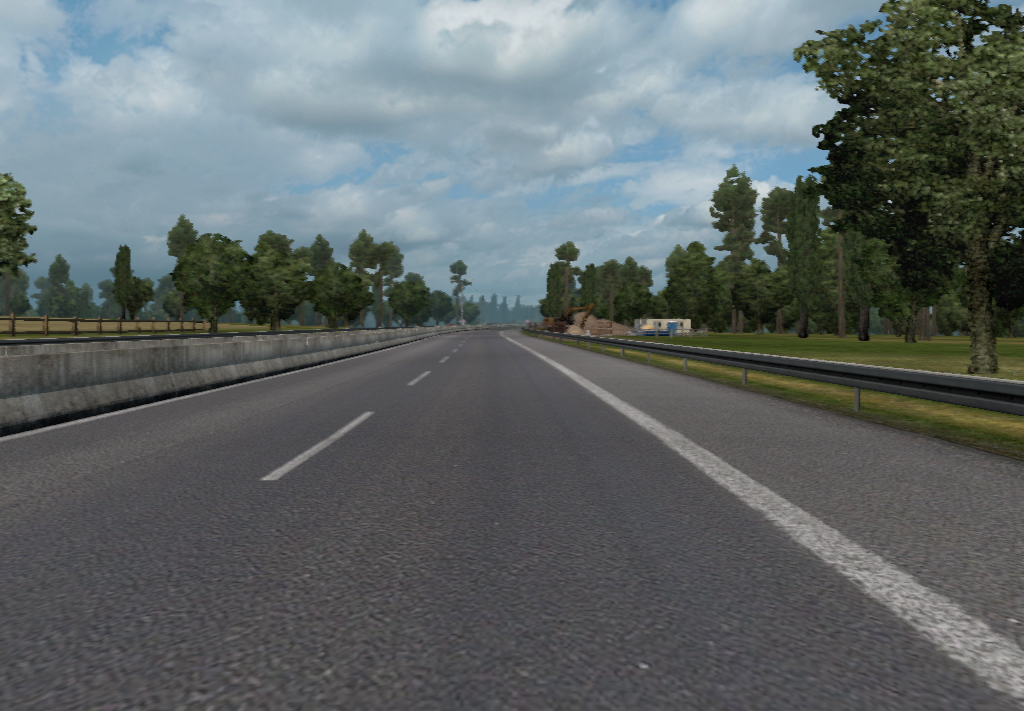
\includegraphics[width=12cm]{img/input.png}
  \caption{Przykładowy obraz wejściowy algorytmu detekcji pasa ruchu}
  \label{fig:inputimg}
  % https://pl.wikipedia.org/wiki/Tesla_Model_S#/media/Plik:2014_Tesla_Motors_Model_S_(rear_view)_Netherlands.jpg
\end{figure}

W najczęstszym przypadku obrazem wejściowym do algorytmu jest obraz z kamery umieszczonej pod pewnym kątem do nawierzchni zamontowanej w okolicy przedniego zderzaka lub atrapy chłodnicy. W niniejszej pracy, większość przetwarzanych obrazów pochodzi z symulatora Euro Truck Simulator 2, gry komputerowej, która posiada zaawansowaną grafikę, która przypomina otaczającą rzeczywistość, a także udostępnia możliwości programistyczne, które ułatwią stworzenie aplikacji do testowania algorytmów wizyjnych co jest założeniem niniejszej pracy. W niniejszej sekcji zostanie opisany algorytm z artykułu \cite{T3}
Autor korzysta w nim z podstawowych operacji przetwarzania obrazów. 



\begin{figure}
  \centering
  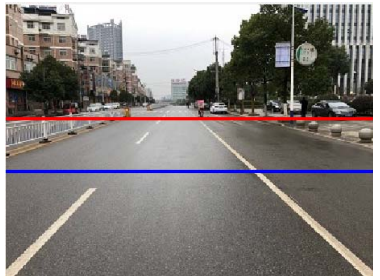
\includegraphics[width=10cm]{img/roi.png}
  \caption{Linie obrazujące granice obszaru poddawanego analizie\cite{T3}}
  \label{fig:roi}
  % artykuł
\end{figure}
Pierwszym krokiem jest wyodrębnienie z obrazu ROI \footnote{ROI (ang.) - Region of interest - obszar obrazu poddawany analizie i dalszemu przetwarzaniu}. Ma to na celu ograniczenie ilości danych poddawanych analizie, a co bardziej istotne odrzuca te fragmenty obrazu, na których na pewno nie będzie jezdni (powyżej czerwonej linii), a także te gdzie obraz linii mógłby być zakłócony. Warto zauważyć, że pomiędzy liniami - czerwoną i niebieską znajduje się prawie dwa razy więcej długości drogi niż w obszarze pod niebieską linią.

Kolejnym etapem jest ekstrakcja pasów ruchu. W większości krajów mają one kolor biały, rzadziej żółty. Są to kolory, które na drodze można rzadko zauważyć w innej funkcji niż malowanie znaków poziomych, w tym linii. Mając na wejściu obraz RGB\footnote{RGB - obraz o trzech składowych barwnych czerwonej(R), zielonej(G) i niebieskiej(B)} można zauważyć, że składowe czerwona i zielona mają większe wartości tam gdzie na obrazie są linie w porównaniu do standardowej nawierzchni jezdni. W artykule, który opisuje ta sekcja zaproponowano następującą metodę segmentacji linii:
\begin{equation}
\label{eq:IMij}
IM(i,j)=\left\{\begin{matrix}
255, & \begin{matrix}
R(i,j)\geq (0.2R_{min}+0.8R_{max})\\ 
G(i,j)\geq (0.2G_{min}+0.8G_{max})
\end{matrix}\\ 
0, & wpp\footnote{w przeciwnym przypadku}.
\end{matrix}\right.
\end{equation}

\begin{equation}
\label{eq:Gij}
G(i,j)=\left\{\begin{matrix}
255, & \begin{matrix}
R(i,j)\geq G(i,j) \geq B(i,j)\\ 
IM(i,j)>0
\end{matrix}\\ 
0, & wpp.
\end{matrix}\right.
\end{equation}

\begin{equation}
\label{eq:Gray}
Gray(i,j)=R(i,j)+G(i,j)-2B(i,j)+0.3*8|R(i,j)+G(i,j)|
\end{equation}

\begin{equation}
\label{eq:GMij}
GM(i,j)=\left\{\begin{matrix}
128, &  Gray(i,j)\geq 0.8*Gray_{m} \\ 
255, & \begin{matrix}
2*Gray_{avg} \leq Gray(i, j) \leq Gray_{m}\\albo\\ 
G(i,j)=255
\end{matrix} \\ 
0,   & wpp.
\end{matrix}\right.
\end{equation}

W równaniu \eqref{eq:IMij} \ ${IM(i,j)}$ oznacza tymczasową macierz cech koloru. ${R(i,j)}$ oznacza jasnośc składowej czerwonej, a ${G(i,j)}$ składową zieloną. ${R_{max}}$, ${R_{min}}$, ${G_{max}}$, ${G_{min}}$ reprezentują maksymalną i minimalną wartość składowej czerwonej, a także maksymalną i minimalną wartość składowej zielonej. W równaniu \eqref{eq:Gray} \ $ Gray(i,j)$ wskazuje na obraz wejściowy w skali szarości, na wartości którego ma wpływ każda ze składowych barwnych. W ostatnim równaniu \eqref{eq:GMij} \ $GM(i,j)$ oznacza obraz wynikowy, na którym zaznaczone jest wysegmentowane poziome oznaczenie jezdni. $Gray_{avg}$ to średnia wartość obrazu w skali szarości w danym wierszu, natomiast $Gray_{m}(i,j)$ oznacza wartość maksymalną dla danego wiersza.

\begin{figure}
  \centering
  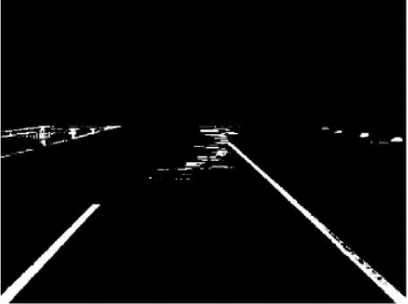
\includegraphics[width=7cm]{img/segmentacja.png}
  \caption{Obraz $GM$ -- wysegmentowane linie\cite{T3}}
  \label{fig:segmented}
  % https://pl.wikipedia.org/wiki/Tesla_Model_S#/media/Plik:2014_Tesla_Motors_Model_S_(rear_view)_Netherlands.jpg
\end{figure}


Kolejnym etapem opisywanego algorytmu jest wykrywanie krawędzi, tu zrealizowane za pomocą filtru Canny'ego. Jest to filtr nieliniowy z histerezą. Dobrze sprawdza się do wykrywania krawędzi na obrazach niejednorodnych i rozmytych. Następnie podejmowana jest ekstrakcja cech linii. Na potrzeby wyjaśnienia działania podanego fragmentu algorytmu przyjęto:
\begin{itemize}
\item $IME$ -- Obraz z równania \eqref{eq:GMij} po filtracji filtrem Canny'ego
\item $IMC$ -- Obraz $GM$ z równania \eqref{eq:GMij}
\end{itemize}

Dla każdego piksela w obrazie $IME$ który został oznaczony jako krawędź zostaje sprawdzana następująca zależność:
\begin{equation}
	\begin{matrix}
	IMC(i,j+1)+IMC(i,j)+IMC(i,j-1)+IMC(i-1,j+1)\\
	+IMC(i-1,j)+IMC(i-1,j-1)+IMC(i+1,j+1)+IMC(i+1,j-1)>0
	\end{matrix}
\end{equation}
Jeśli jest ona spełniona, wybrany punkt na obrazie $IME$ zostaje uznany jako krawędź pasa jezdni.

\begin{figure}
  \centering
  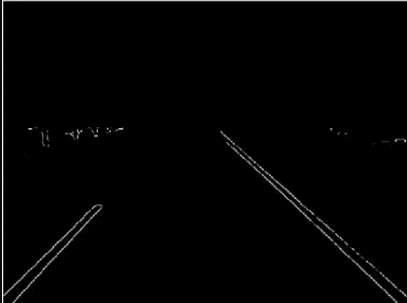
\includegraphics[width=7cm]{img/canny.png}
  \caption{Obraz po zastosowaniu filtra Canny'ego oraz ekstrakcji cech linii\cite{T3}}
  \label{fig:canny}
  % https://pl.wikipedia.org/wiki/Tesla_Model_S#/media/Plik:2014_Tesla_Motors_Model_S_(rear_view)_Netherlands.jpg
\end{figure}

Do ostatecznego wykrycia linii prostych należy użyć zmodyfikowanej transfomaty Hougha( \textit{constraint Hough transform}). Główna różnica pomiędzy nią, a klasyczną transformatą Hougha polega na tym, że wartości $\rho$ i $\theta$ są skwantowane i pogrupowane. Dzięki takiej modyfikacji linie które leżą blisko siebie lub w przypadku nieidalnie prostej linii redukuje się prawdopodobieństwo wielokrotnej detekcji prostej.

\begin{figure}
  \centering
  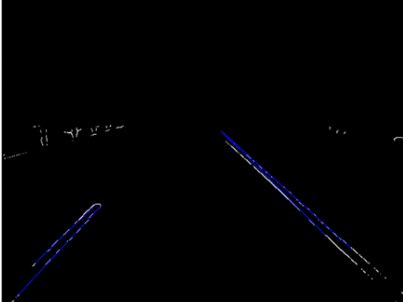
\includegraphics[width=7cm]{img/prehough.png}
  \caption{Wynik algorytmu detekcji linii\cite{T3}}
  \label{fig:result}
  % https://pl.wikipedia.org/wiki/Tesla_Model_S#/media/Plik:2014_Tesla_Motors_Model_S_(rear_view)_Netherlands.jpg
\end{figure}

\subsection{Detekcja zakrętów}
Podobnym zadaniem jest detekcja pasa ruchu w zakręcie. Kształt zakrzywionej linii może być opisany za pomocą paraboli z równania \ref{eq:ld_1}. Zauważono, że fragment drogi bliżej samochodu z reguły jest prosty, zakrzywienie widać powyżej pewnej odległości, a na obrazie powyżej pewnej wysokości. Równanie \ref{eq:ld2} pokazuje model pasa ruchu, gdzie $y_m$ to współrzędna punktu, w którym prosta przechodzi w krzywą.
\begin{equation}
x=a+by+cy^{2}
\end{equation}

\begin{equation}
x=\begin{cases}
a+by,\qquad\qquad y\leq y_{m}\\ c+dy+ey^{2},\qquad y > y_{m} \end{cases}
\end{equation}

gdzie ponadto:
\begin{itemize}
\item $a,b$ -- parametry linii
\item $c,d,e$ -- parametry krzywej
\end{itemize}

Linie prosta i krzywa powinny spotykać się w jedym punkcie, którego współrzędna wysokościowa jest równa $y_m$. Po pewnych przekształceniach otrzymano równanie \ref{eq:ld_3} i \ref{eq:ld_4}.

\begin{equation}
a+by_{m}=c+dy_{m}+ey_{m}^{2}
\end{equation}

\begin{equation}
b = d+2ey_m
\end{equation}

Ostatecznie uzyskano zależność \ref{eq:ld_5} pomiędzy parametrami krzywych.

\begin{equation}
\begin{cases} c=a+\frac{y_{m}}{2}(b-d) \\
e=\frac{1}{2y_{m}}(b-d) \end{cases}
\end{equation}


\section{Detekcja znaków drogowych}

Innym w swojej naturze zadaniem stawianym przed systemami wizyjnymi w pojazdach autonomicznych jest detekcja znaków drogowych. Systemy tego typu pojawiały się dość wcześnie w samochodach pełniąc jedynie funkcję ostrzegawczo-informacyjną. Coraz bardziej dynamicznie rozwijające się systemy wspomagające kierowcę wymagają od subsystemu odpowiedzialnego za detekcję znaków drogowych dużej skuteczności, ponieważ na ich detekcjach opierają decyzje o sterowaniu pojazdem. Istotnym problemem jest brak ujednoliconego zestawu znaków dla całego świata. Obecnie każdy kraj posiada swój zestaw znaków, które w ogólności są podobne, jednak różnice w szczegółach sprawiają problemy systemom wizyjnym. Proponowanym rozwiązaniem jest zbudowanie odpowiednio dużej bazy wzorców znaków i stosowanie określonego zestawu w zależności od lokalizacji. 

Rozwiązanie proponowane w \cite{T2} składa się z dwóch etapów. Pierwszy to detekcja znaku, a drugi to jego klasyfikacja. Do wykrycia znaku drogowego na obrazie pochodzącym z kamery umieszczonej w samochodzie użyto \textit{Radial Symmetry Transform} do detekcji znaków ograniczenia prędkości. Obecnie stowane metody detekcji bazują na segmentacji koloru lub kształtu. 

\subsection{Radial Symmetry Transform}
Klasyczne detektory kształtu wymagają często zamkniętych konturów. Odporne techniki takie jak transformata Hougha dla kół wymaga dużych nakładów obliczeniowych dla dużych obrazów. \textit{Fast radial symmetry detector - (ang. Szybki radialny detektor symetrii)} może być używany jako detektor w czasie rzeczywistym. Znakomita większość znaków z ograniczeniem prędkości to koło z czerwonym brzegiem i wartością ograniczenia w środku na białym tle. Opisywana metoda detekcji jest kompatybilna ze wszystkimi głównymi metodami klasyfikacji takimi jak np. SVM (ang. Support Vector Machine - maszyna wektorów wspierających). Główną zaletą użycia opisywanej metody jest fakt, że wraz z informacją o wykrytym znaku podawana jest skala znaku, co znacząco ułatwia klasyfikację, ponieważ niepotrzebne staje się używanie szablonów o wielu rozmiarach dla wielu różnych rozdzielczości.

Szybki radialny detektor symetrii jest wariantem transformaty Hougha dla wyszukiwania okręgów. Jest on wykonywany w porządku $kp$, gdzie $k$ oznacza liczbę promieni, które są szukane, a $p$ liczbę pikseli. Stanowi to różnicę w stosunku do klasycznej transformaty Hougha wykonywanej w porządku $kbp$, gdzie każdy piksel na obrazie krawędzi ,,głosuje'' dla każdego koła z dyskretnego zestawu promieni. $b$ oznacza dyskretyzację zestawu promieni okręgów, które mogą przechodzić przez aktualnie analizowany punkt.

\begin{figure}
  \centering
  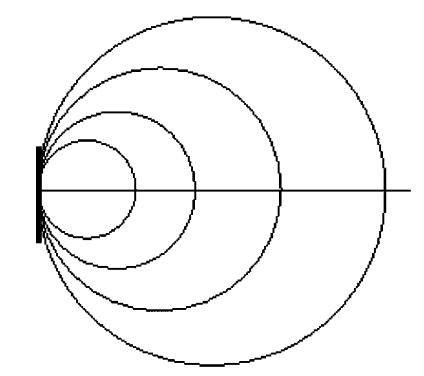
\includegraphics[width=7cm]{img/fsrd1.png}
  \caption{Algorytm głosowania - dla danego punktu krawędzi środki rodziny krawędzi leżą na lini prostopadłej do krawędzi\cite{T2}}
  \label{fig:frsd1}
\end{figure}

FRSD eliminuje czynnik $b$ poprzez pozyzskanie informacji o kierunku gradientu z detektora krawędzi Sobela. Zamiast sprawdzania każdego możliwego kierunku promienia, sprawdzany jest jedynie kierunek prostopadły do kierunku gradientu co jest widoczne na rysunku \ref{fig:frsd1}. Powoduje to, że przestrzeń rozwiązań z trójwymiarowej staje się dwuwymiarowa, co pozwala na używanie algorytmu w czasie rzeczywistym. Operacja radialnej detekcji symetrii może być prosto zrozumiana jako rozważenie wszystkich możliwych okręgów, których dany piksel może być częścią, jeżeli znany jest kierunek krawędzi, to okręgi są szukane tylko na linii prostopadłej do krawędzi (rys. \ref{fig:frsd2}).

\begin{figure}
  \centering
  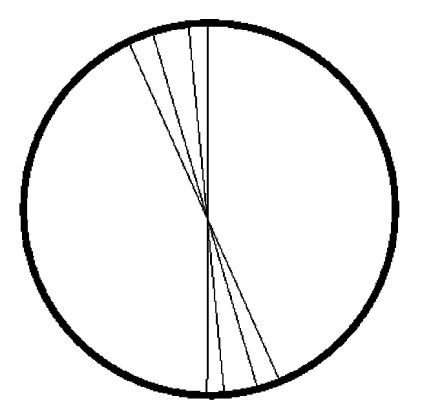
\includegraphics[width=7cm]{img/fsrd2.png}
  \caption{Zachowanie FRSD dla okręgu, zauważalne przecięcie średnic skutkuje istnieniem maksimum lokalnego w środku okręgu.\cite{T2}}
  \label{fig:frsd2}
\end{figure}

Praktyczna realizacja jest wykonywana na obrazie cyfrowym, więc promień jest podzielony na kilka zakresów długości. Istotne jest poprawne dobranie ograniczeń na długość promienia. Na rysunku \ref{fig:tsd} po prawej stronie jest widoczny znak ograniczenia prędkości, który powinien zostać wykryty. Daje się zauważyć, że można dobrać odpowiednie zakresy promienia dla wykrywanych znaków, a także wyodrębnić obszar na którym znaki na pewno nie będą się pojawiać, a także taki, na którym należy wykonać detekcję.
\begin{figure}
  \centering
  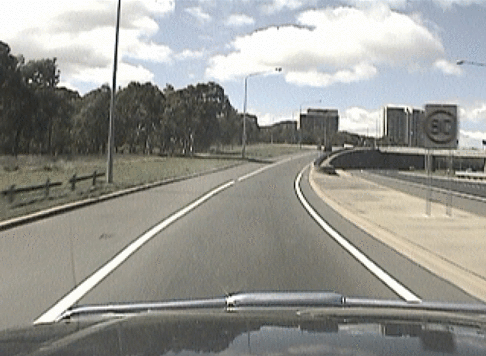
\includegraphics[width=7cm]{img/znaki1.png}
  \caption{Obraz wejściowy algorytmu detekcji znaków drogowych\cite{T2}}
  \label{fig:tsd}
\end{figure}

%\begin{figure}
%\centering
%\subfloat[obraz 1]{\label{fig:znaki2}
%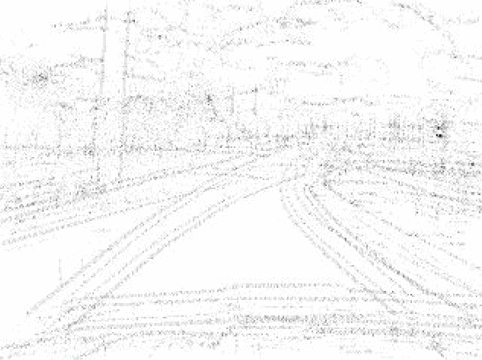
\includegraphics[width=0.3\textwidth]{img/znaki2.png}}
%\quad
%\subfloat[obraz 2]{\label{fig:znaki3}
%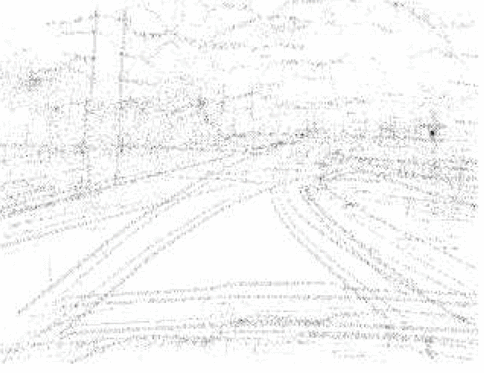
\includegraphics[width=0.3\textwidth]{img/znaki3.png}}
%\caption{Wyniki detekcji, gdy zakres promieni jest zbyt mały \protect\subref{subfigure_a} i zbyt duży, \protect\subref{subfigure_b}.}
%\label{fig:tsd1}
%\end{figure}

\begin{figure}[h]
	\centering
	\begin{subfigure}{0.35\textwidth}
		\centering
		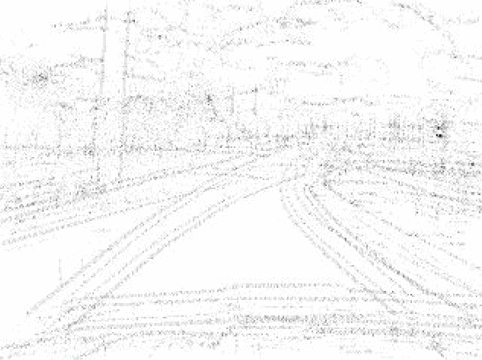
\includegraphics[width=6cm]{img/znaki2.png}
		\subcaption{\label{fig:znaki2}}
	\end{subfigure}
	\begin{subfigure}{0.35\textwidth}
		\centering
		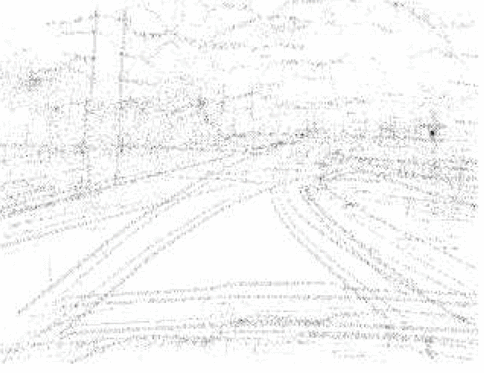
\includegraphics[width=6cm]{img/znaki3.png}
		\subcaption{\label{fig:znaki3}}
	\end{subfigure}
	
	\caption{\label{fig:details}Wyniki detekcji, gdy zakres promieni jest zbyt mały \protect\subref{fig:znaki2} i zbyt duży \protect\subref{fig:znaki3}.\cite{T2}}
\end{figure}

\section{Detekcja świateł drogowych}
\label{sec:tl}
Kolejnym istotnym elementem systemów umieszczanych w pojazdach autonomicznych jest detekcja świateł drogowych. Informują one o możliwości przejazdu przez skrzyżowanie lub rondo i możliwości znalezienia się na trasie kolizyjnej w stosunku do innych użytkowników drogi. Światła drogowe spotykane są głównie w miastach, lecz wraz z rozwojem infrastruktury widywane są w mniejszych miejscowościach. Słupy z zamontowanymi światłami mogą być widoczne na prawej lub lewej krawędzi jezdni, a także nad nią.

\subsection{Detekcja świateł drogowych z użyciem informacji o kolorze i krawędziach}
Światła drogowe na świecie są ustandaryzowane. Istnieją trzy kolory: czerwony, żółty i zielony. Każdy kolor niesie za sobą informację: czerwony - stój, żółty - przygotuj się do zmiany z zielonego na czerwony lub odwrotnie i zielony, który oznacza jedź. Jedyną znaną odchyłką jest odpowiednik światła żółtego w Stanach Zjednoczonych, który jest pomarańczowy.

\begin{figure}
  \centering
  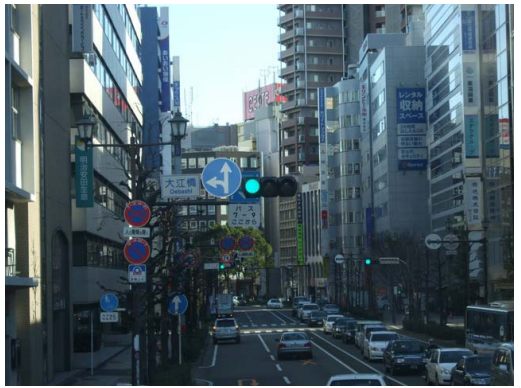
\includegraphics[width=7cm]{img/tl_input.png}
  \caption{Obraz wejściowy algorytmu detekcji świateł drogowych\cite{T4}}
  \label{fig:tl_input}
\end{figure}

Masako Omachi w artykule \cite{T4} proponuje algorytm, który bazuje na informacji o kolorze i krawędzi znajdujących się na obrazie. Światła drogowe mają z góry ustalony kształt - są okrągłe. Istnieją warianty ze strzałkami, lecz opisywany poniżej algorytm służy do detekcji świateł, które w \cite{Kodeks} mają kształ pełnego koła.

Rysunek \ref{fig:tl_input} pokazuje przykład sceny zawierającej światła drogowe. W opisywanej metodzie przestrzeń barw jest konwertowan do znormalizowanej przestrzeni RGB. Normalizacja przestrzeni RGB polega na zmapowaniu wartości pikseli do przedziału $[0,255]$. A także ,,rozsunięciu'' wartości pikseli na obrazie tak, by znajdowały się w całym możliwym zakresie wartości:
\begin{equation}
R=\left\{\begin{matrix}
0, &  s=0\\
\frac{r}{s} & w p.p.
\end{matrix}\right.
\end{equation}
\begin{equation}
G=\left\{\begin{matrix}
0, &  s=0\\
\frac{g}{s} & w p.p.
\end{matrix}\right.
\end{equation}
\begin{equation}
B=\left\{\begin{matrix}
0, &  s=0\\
\frac{b}{s} & w p.p.
\end{matrix}\right.
\end{equation}
gdzie:
\begin{itemize}
\item$r,g,b$ -- składowe czerwona, zielona i niebieska nieznormalizowanego obrazu,
\item$s = r+g+b$
\item$R,G,B$ -- składowe czerowna, zielona i niebieska znormalizowanego obrazu.
\end{itemize}


\begin{figure}
  \centering
  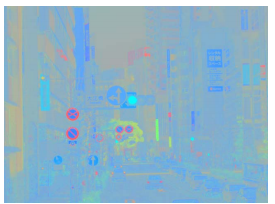
\includegraphics[width=7cm]{img/tl_norm.png}
  \caption{Efekt normalizacji przestrzeni barw\cite{T4}}
  \label{fig:tl_norm}
\end{figure}

Efekt przeniesienia przestrzeni barw do znormalizowanej przestrzeni RGB jest widoczny na rysunku \ref{fig:tl_norm}.
Następnie poprzez progowanie każdej ze składowych uzyskuje się kandydatów do detekcji świateł drogowych. Decyzja o tym czy piksel neleży lub nie do światła drogowego jest podejmowana na podstawie poniższych warunków:
\begin{equation}
R>200 \wedge G< 150 \wedge B<150
\end{equation}
lub
\begin{equation}
R>200 \wedge G> 150 \wedge B<150
\end{equation} 
lub
\begin{equation}
R<150 \wedge G>240 \wedge B>220
\end{equation}.

\begin{figure}
  \centering
  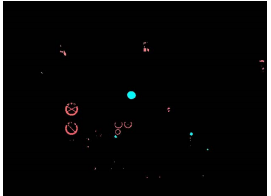
\includegraphics[width=7cm]{img/tl_thresh.png}
  \caption{Rezultat progowania w celu wykrycia obszarów będących kandydatami do bycia światłami drogowymi\cite{T4}}
  \label{fig:tl_thresh}
\end{figure}

Rezultat progowania jest widoczny na rysunku \ref{fig:tl_thresh}. Następnym krokiem jest wykrycie krawędzi na obrazie z kandydatami do detekcji świateł. Jedną z opcji jest użycie filtru Sobela. Ostatnim etapem, jako, że światła drogowe mają jasno określony kształt jest użycie transformaty Hougha dla okręgów, by wykryć właściwe światła drogowe. W artykule stosowana jest zmodyfikowana transformata Hougha do wyszukiwania okręgów, która polega na ustaleniu stałej długości promienia. Klasyczna transformata Hougha jest opisana w sekcji \ref{sec:vision_algs}.

\subsection{Wnioski i rezultaty}
Opisany algorytm detekcji świateł drogowych daje lepsze wyniki niż użycie standardowej przestrzeni barw i klasycznej transformaty Hougha dla okręgów. Porównanie jest zamieszczone w tabeli \ref{tab:tl_results}. Główną zaletą opisywanej metody detekcji świateł drogowych jest fakt, że poprawnie odrzuca ona obrazy znaków drogowych, które również mają okrągłe kształy i jednolite kolory na krawędziach. Algorytm bierze dodatkowo pod uwagę czy kolor na krawędziach jest taki sam jak wewnątrz kształtu, co pozwala skutecznie odrzucić np. znaki zakazu.
Problemem, który napotyka algorytm są tylne światła innych pojazdów, które mają jednolity kolor (z reguły czerwony), a także kształt zbliżony do czerwonego. Przykładowy błąd detekcji jest ukazany na rysunku \ref{fig:tl_err}.

\begin{figure}
  \centering
  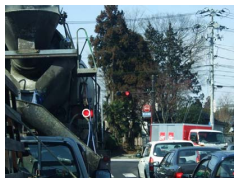
\includegraphics[width=7cm]{img/tl_err.png}
  \caption{Przykład błędnej detekcji tylnego światła traktora\cite{T4}}
  \label{fig:tl_err}
\end{figure}

\begin{table}[]
\centering
\caption{Porównanie klasycznego algorytmu detekcji świateł i opisanego w tej pracy\cite{T4}}
\begin{tabular}{lllll}
\cline{1-3}
\multicolumn{1}{|l|}{}                           & \multicolumn{1}{l|}{Algorytm klasyczny} & \multicolumn{1}{l|}{Algorytm opisany w tym rozdziale} &  &  \\ \cline{1-3}
\multicolumn{1}{|l|}{Dokładność}                 & \multicolumn{1}{l|}{20/30}              & \multicolumn{1}{l|}{26/30}                            &  &  \\ \cline{1-3}
\multicolumn{1}{|l|}{Czas przetwarzania {[}s{]}} & \multicolumn{1}{l|}{0.561}              & \multicolumn{1}{l|}{0.347}                            &  &  \\ \cline{1-3}
                                                 &                                         &                                                       &  & 
\end{tabular}
\label{tab:tl_results}
\end{table}



\section{Detekcja samochodu poprzedzającego}
\label{sec:car_general}
Istotnym zadaniem stawianym przed algorytmami wizyjnymi stosowanymi w pojazdach autonomicznych jest detekcja samochodów w najbliższym otoczeniu pojazdu. Detekcja może być wspierana odczytami z radaru lub lidaru, jednak w poniższej sekcji zostanie opisany algorytm bazujacy jedynie na obrazie z kamer. Większość współczesnych samochodów widzianych od tyłu zachowuje symetrię wględem pionowej osi przechodzącej przez środek pojazdu. 

Pierwszym wstępnym krokiem jest zbadanie możliwych pozycji samochodów na obrazie i oznaczenie ich jako ROI. Dla systemu z fuzją danych wizyjnych i radarowych, może to być zrobione poprzez poprzez analizę odległości i prędkości względnej, czyli danych uzyskanych z radaru. Dla systemu, który posiada jedną kamerę pozycja samochodów musi być wyznaczona tylko na podstawie ruchu samochodów na obrazie w czasie.

Opisywany algorytm korzysta z detektora symetrii, który działa w następujący sposób. Dla każdego piksela wyznaczana jest liczba punktów, która jest wartością bezwzględną z różnicy wartości pikseli, które są równoodległe od ustalonej osi symetrii. Jest to zwykle robione z użyciem pewnego okna o z góry ustalonym rozmiarze dobieranym tak, aby pasować do rozmiaru samochodów, które mogą znajdować się na obrazie. Będąc świadomym faktu, że samochód im jest dalej od kamery, tym jest mniejszy zastosowano kilka predefiniowanych rozmiarów okien. Wartości wskaźnika symterii mogą być obliczne dla każdego punktu na obrazie. Piksele z dużą jego wartością są dobrymi kandydatami do należenia do osi symetrii. Wyliczanie wskaźnika symetrii dla każdego punktu na obrazie jest bardzo czasochłonne, więc zdecydowano się na jego wyznaczanie tylko na wcześniej określonych poziomych liniach, które z grubsza pokrywają obszar, na którym mogą znajdować się samochody. Do obliczania wskaźnika symetrii może być użytych kilka cech obrazu takich jak: wartości pikseli w skali szarości, obraz krawędzi, składowa S w przestrzeni barw HSV. Szukanie obrazu samochodu na obrazie w skali szarości jest szybsze, jednak wrażliwe na na zmiany oświetlenia (noc, deszcz). Dobrze sprawdza się badanie nasycenia w przestrzeni barw HSV, ponieważ uniezależnia to obraz samochodu od ogólnej jasności otoczenia i częściowo od pogody.

\subsection{Przebieg algorytmu bazującego na operatorze symetrii}
Pierwszym krokiem jest wygenerowanie obrazu krawędzi na podstawie obrazu w skali szarości lub składowej S przestrzeni barw HSV. W opisanym algorytmie zaproponowano detektor Canny'ego. Rysunek \ref{fig:car_edge} pokazuje rezultat wykrywania krawędzi dla typowego obrazu zawierającego samochód poprzedający. Opierając się na znanej pozycji kamery i jej pochyleniu względem nawierzchni drogi można określić obszar na obrazie, na którym będą szukane samochody. Poziome ograniczenia znajdują się pomiędzy horyzontem i początkiem widocznej drogi na dole obrazu. Pionowe ograniczenia są ustawione tak, by odpowiadać lewemu i prawemu ograniczeniu jezdni. 

\begin{figure}
  \centering
  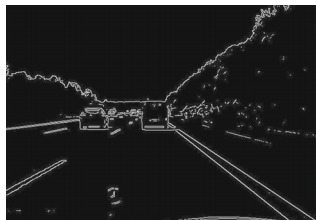
\includegraphics[width=7cm]{img/car_canny.png}
  \caption{Obraz z samochodami po filtracji filtrem Canny'ego\cite{T1}}
  \label{fig:car_edge}
\end{figure}

Jak wspomniano w sekcji \ref{sec:car_general}, w celu zredukowania czasu obliczeń nie każdy piksel w wybranym obszarze jest analizowany. Obliczenia dotyczące symetrii są przeprowadzane tylko dla 15 równoodległych linii skanu (rys. \ref{fig:car_scan_lines1}). Wejściowa rozdzielczość obrazu nie ma znaczenia dla obliczeń. Dzieje się tak ponieważ algorytm wykrywa tylko maksima wzdłuż linii skanu.

\begin{figure}
  \centering
  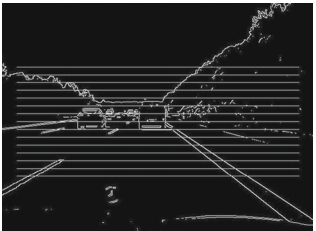
\includegraphics[width=7cm]{img/car_lines.png}
  \caption{Obraz z samochodami po filtracji filtrem Canny'ego i zaznaczonymi liniami skanu\cite{T1}}
  \label{fig:car_scan_lines1}
\end{figure}

Kolejnym krokiem jest detekcja symetrii. Jest ona przeprowadzana dla każdego punktu leżącego na linii skanu. Wartość operatora symetrii dla piksela wyraża się wzorem:

\begin{equation}
SymVal(x,y)=\sum_{x'=1}^{W/2}\sum_{y'=y-H/2}^{y+H/2}S(x, x', y')
\end{equation}
gdzie:
\begin{itemize}
\item
\begin{equation}
S(x,x',y')=\begin{cases}
2 & \text{ gdy } I(x-x',y')=I(x+x',y')=1 \\ 
-1 & \text{ gdy } I(x-x',y')\neq I(x+x',y') \\ 
0 & \text{ w p.p. }
\end{cases}
\end{equation}
\item $W$ -- szerokość okna
\item $H$ -- wysokość okna
\item $I(x,y)$ -- wartość piksela o współrzędnych $x,y$
\end{itemize}

Szerokość okna powinna być właściwie ustawiona, aby poprawnie wykrywać symetryczne obiekty o różnych rozmiarach. W trakcie eksperymentów wykazano, że optymalne wartości $W$ mieszczą się w przedziale $[8,12]$.

\begin{figure}
  \centering
  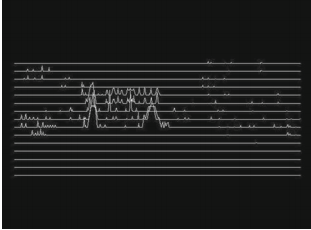
\includegraphics[width=7cm]{img/tl_peaks.png}
  \caption{Wartości wskaźnika symetrii wyznaczone dla linii skanu\cite{T1}}
  \label{fig:car_scan_lines}
\end{figure}

Na rysunku \ref{fig:car_scan_lines} widać, że w niektórych punktach istnieją maksima, które wskazują, że dany punkt może należeć do osi symetrii. Wybiera się maksima i stosuje progowanie, to znaczy wartości maksimów lokalnych poniżej pewnej wartości są odrzucane. Zwykle wartości poniżej określonego progu wskazują na małe, symetryczne elementy tła. Progowania dokonuje się według następującej formuły:
\begin{equation}
SymPts(x,y)=\begin{cases}
1 & \text{ gdy } SymVal(x,y)>T\\ 
0 & \text{ w p.p.}
\end{cases}
\end{equation}

gdzie
\begin{itemize}
\item $T$ - ustalony próg odrzucenia maksimum lokalnego
\end{itemize}


\begin{figure}
  \centering
  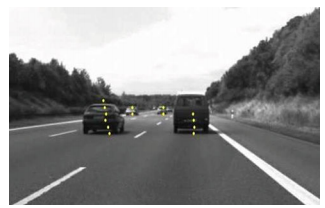
\includegraphics[width=7cm]{img/car_symmetry.png}
  \caption{Wykryte osie symetrii na liniach skanu\cite{T1}}
  \label{fig:car_detected}
\end{figure}

Ostatecznie znalezione maksima oznaczają wykryte osie symetrii względnie dużych obiektów, w tym przypadku samochodów. Widać to na rysunku \ref{fig:car_detected}. Dla każdej linii skanu wykryta oś symetrii jest przesunięta o kilka pikseli, dlatego ostatnim etapem detekcji samochodu jest klasteryzacja.

Uzyskane punkty osi symetrii są klasteryzowane metodą k-średnich. Liczba samochodów na obrazie jest nieznana, więc klasteryzację robi się iteracyjnie, co iterację licząc wariancję, która przy poprawnej liczbie klastrów w stosunku do samochodów na obrazie będzie mniejsza niż określony próg. Końcowy wynik z zaznaczonymi środkami samochodów jest widoczny na rysunku \ref{fig:car_end}

\begin{figure}
  \centering
  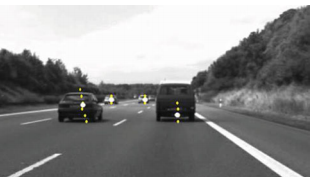
\includegraphics[width=7cm]{img/car_end.png}
  \caption{Wynik algorytmu detekcji samochodów poprzedających\cite{T1}}
  \label{fig:car_end}
\end{figure}

\section{Opis wybranych zagadnień i algorytmów przetwarzania obrazu}
\label{sec:vision_algs}
W tej sekcji zostaną opisane podstawowe algorytmy i zagadanienia dotyczące cyfrowego przetwarzania obrazów, które są używane w zaawansowanych algorytmach wizyjnych w pojazdach autonomicznych.

\subsection{Transformata Hougha dla okręgów}

Systemy wizyjne w pojazdach autonomicznych często mają za zadanie wykrycie obiektów o kształcie koła. Algorytmem do tego przeznaczonym jest transformata Hougha. Istnieje ona w wersji do detekcji prostych i okręgów. Pod pojęciem uogólniona transformata Hougha kryje się algorytm służący do detekcji dowolnego zadanego konturu.

Okrąg można sparametryzować za pomocą następującego wzoru:
\begin{equation}
(x-x_0)^2+(y-y_0)^2=r^2
\end{equation}
gdzie
\begin{itemize}
\item $x_0, y_0$ -- współrzędne środka okręgu
\item $r$ -- promień okręgu
\end{itemize}

\begin{figure}[h]
\centering
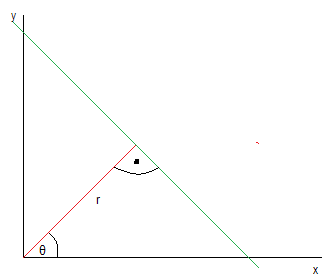
\includegraphics[width=7cm]{img/hough.png}
\caption{Linia w układzie współrzędnych określona za pomocą parametrów $(r, \theta)$}
\label{fig:hough}
\end{figure}

Jeżeli promień będzie ustalony,to okrąg zostanie sparametryzowany za pomocą dwóch liczb. Gdy szukamy okręgów o nieznanych promieniach, rośnie złożoność obliczeniowa, ponieważ wymiar przestrzeni parametrów zwiększa się o jeden.

Możliwa jest również parametryzacja okręgu w biegunowym układzie współrzędnych:
\begin{equation}
x = x_0 + rcos(\theta)
\end{equation}
\begin{equation}
y = y_0 + rsin(\theta)
\end{equation}

po prostym przekształceniu orzymano:

\begin{equation}
x_0 = x - rcos(\theta)
\end{equation}
\begin{equation}
y_0 = y - rsin(\theta)
\end{equation}

Następnie wyznaczana jest przestrzeń Hougha, w której dla każdego piksela obrazu wyznacza się liczbę możliwych okręgów do których mógłby należeć. Wartości maksymalne w przestrzeni Hougha oznaczają wykryty okrąg.

\subsection{Przestrzenie barw}

Podstawową przestrzenią barw jest RGB. Przestawiona na rysunku \ref{fig:rgb} za pomocą sześcianu. Każda składowa jest odpowiedzialna za informację o zawartości danego koloru. Jej zaletą jest prostota opisu, natomiast wadą jest fakt, że po niewielkiej zmianie wartościskłądowych otrzymuje się zupełnie inną barwę. Dodatkowo, co jest ważne w przypadku systemów wizyjnych, niewielka zmiana poziomu jasności powoduje duże wahania składowych R, G, B.

\begin{figure}
  \centering
  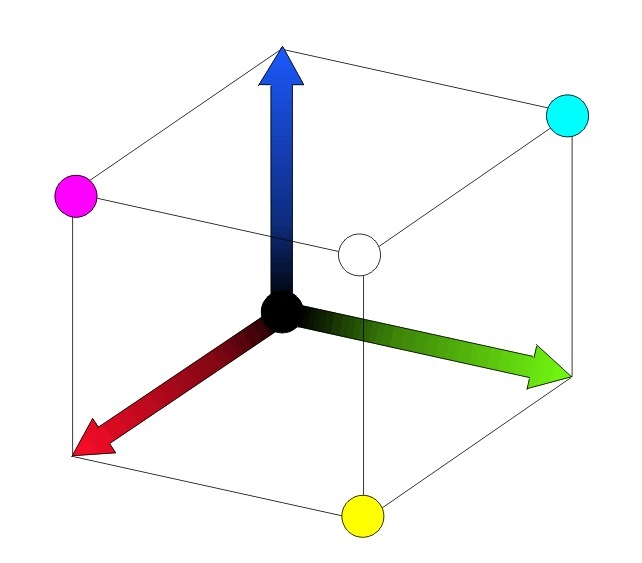
\includegraphics[width=7cm]{img/rgb.jpg}
  \caption{Sześcian przedstawiający przestrzeń barw RGB\cite{W4}}
  \label{fig:rgb}
\end{figure}


\begin{figure}
  \centering
  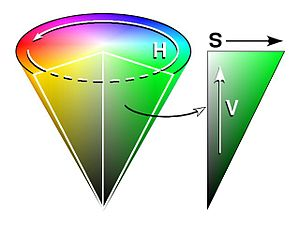
\includegraphics[width=7cm]{img/hsv.jpg}
  \caption{Stożek przedstawiający przestrzeń barw HSV(\textit{źródło: Wikipedia})}
  \label{fig:hsv}
\end{figure}

Drugą, ważną przestrzenią barw używaną w cyfrowym przetwarzaniu obrazów jest przestrzeń HSV. Przedstawiona na rysunku \ref{fig:hsv} za pomocą stożka. Główną zaletą jest to, że przy niewielkich zmianach jasności są bardzo nieduże zmiany w składowej S. Pozwala to na uniezależenienie się w pewnym stopniu od czynników takich jak pora dnia lub pogoda.

\subsection{Filtr Canny'ego}
Podstawowym, dobrze sprawdzającym się detektorem krawędzi jest filtr Canny'ego. Cechuje się właściwościami:

\begin{itemize}
\item niska liczba fałszywych detekcji krawędzi,
\item poprawne wskazywanie pozycji krawędzi. Pozycja krawędzi wskazywana przez detektor powinna odpowiadać jej prawdziwemu położeniu
\item jedna wykryta krawędź przypadająca na rzeczywistą krawędź
\end{itemize}

Detektor krawędzi Canny'ego jest algorytmem wieloetapowym:
\begin{enumerate}
\item Usunięcie z obrazu jakichkolwiek szumów. Używany jest filtr Gaussa. Przykładowa macierz filtru pokazana jest na rysunku \ref{fig:canny_gauss}
\begin{figure}[h]
\centering
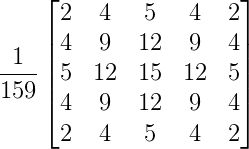
\includegraphics[scale=0.8]{img/canny_gauss.png}
\caption{Maska filtru Gaussa stosowana w wykrywaniu krawędzi}
\label{fig:canny_gauss}
\end{figure}
\item Wyszukiwanie krawędzi z użyciem filtru Sobela o poziomej i pionowej orientacji
\item Określenie wartości gradientu i jego kierunku:

\begin{equation}
G=\sqrt{G_x^2+G_y^2}
\end{equation}

\begin{equation}
\theta=arctan(\frac{G_y}{G_x})
\end{equation}
Kierunek jest zaokrąglany do jednego z czterech możliwych kierunków: \ang{0}, \ang{45}, \ang{90}, \ang{135}

\item Wartości gradientu o niemaksymalnych wartościach są usuwane. Ma to na celu usunięcie pikseli, które prawdopodobnie nie są elementem krawędzi. W wyniku tej operacji pozostają tylko cienkie linie jako krawędzie.

\item Filtr Canny'ego jako argumenty otrzymuje dwa progi - górny i dolny:
\begin{itemize}
\item jeżeli wartość gradientu przekracza górny próg, piksel jest zawsze uznawany jako krawędź
\item jeżeli wartość gradientu nie przekracza dolnego progu, piksel nie jest uznawany za krawędź
\item jeżeli wartość gradientu jest pomiędzy dwoma progami, jest krawędzią, tylko wtedy gdy jest połączony z pikselem, który został sklasyfikowany jako krawędź
\end{itemize}
Twórca filtru rekomenduje stosunek progów filtru pomiędzy 2:1 i 3:1
\end{enumerate}